\documentclass{article}
\usepackage[utf8]{inputenc}

\title{Informe Bases de datos}
\date{April 2015}

\usepackage{natbib}
\usepackage{graphicx}
\usepackage{caratula}
\usepackage[spanish]{babel}


\begin{document}


%%%%%%%%%%%%%%%%%%%%%%%%%%%
%			INICIO DE CARÁTULA			%
%%%%%%%%%%%%%%%%%%%%%%%%%%%

\materia{Bases de datos}
\submateria{Primer Cuatrimestre de 2015}
\titulo{Trabajo Práctico 1}

\grupo{Grupo}
\integrante{Román Gorojovsky}{530/02}{rgorojovsky@gmail.com}

\begin{titlepage}
\maketitle
\thispagestyle{empty}
\end{titlepage} 

\tableofcontents

%%%%%%%%%%%%%%%%%%%%%%%%%%%
%				FIN DE CARÁTULA			%
%%%%%%%%%%%%%%%%%%%%%%%%%%%
\section{Modelado del problema}
\subsection{DER}
A continuación, el diagrama de entidades y sus relaciones para la solución propuesta.
%% INCLUDE PDF
\begin{figure}[h!]
  \centering
    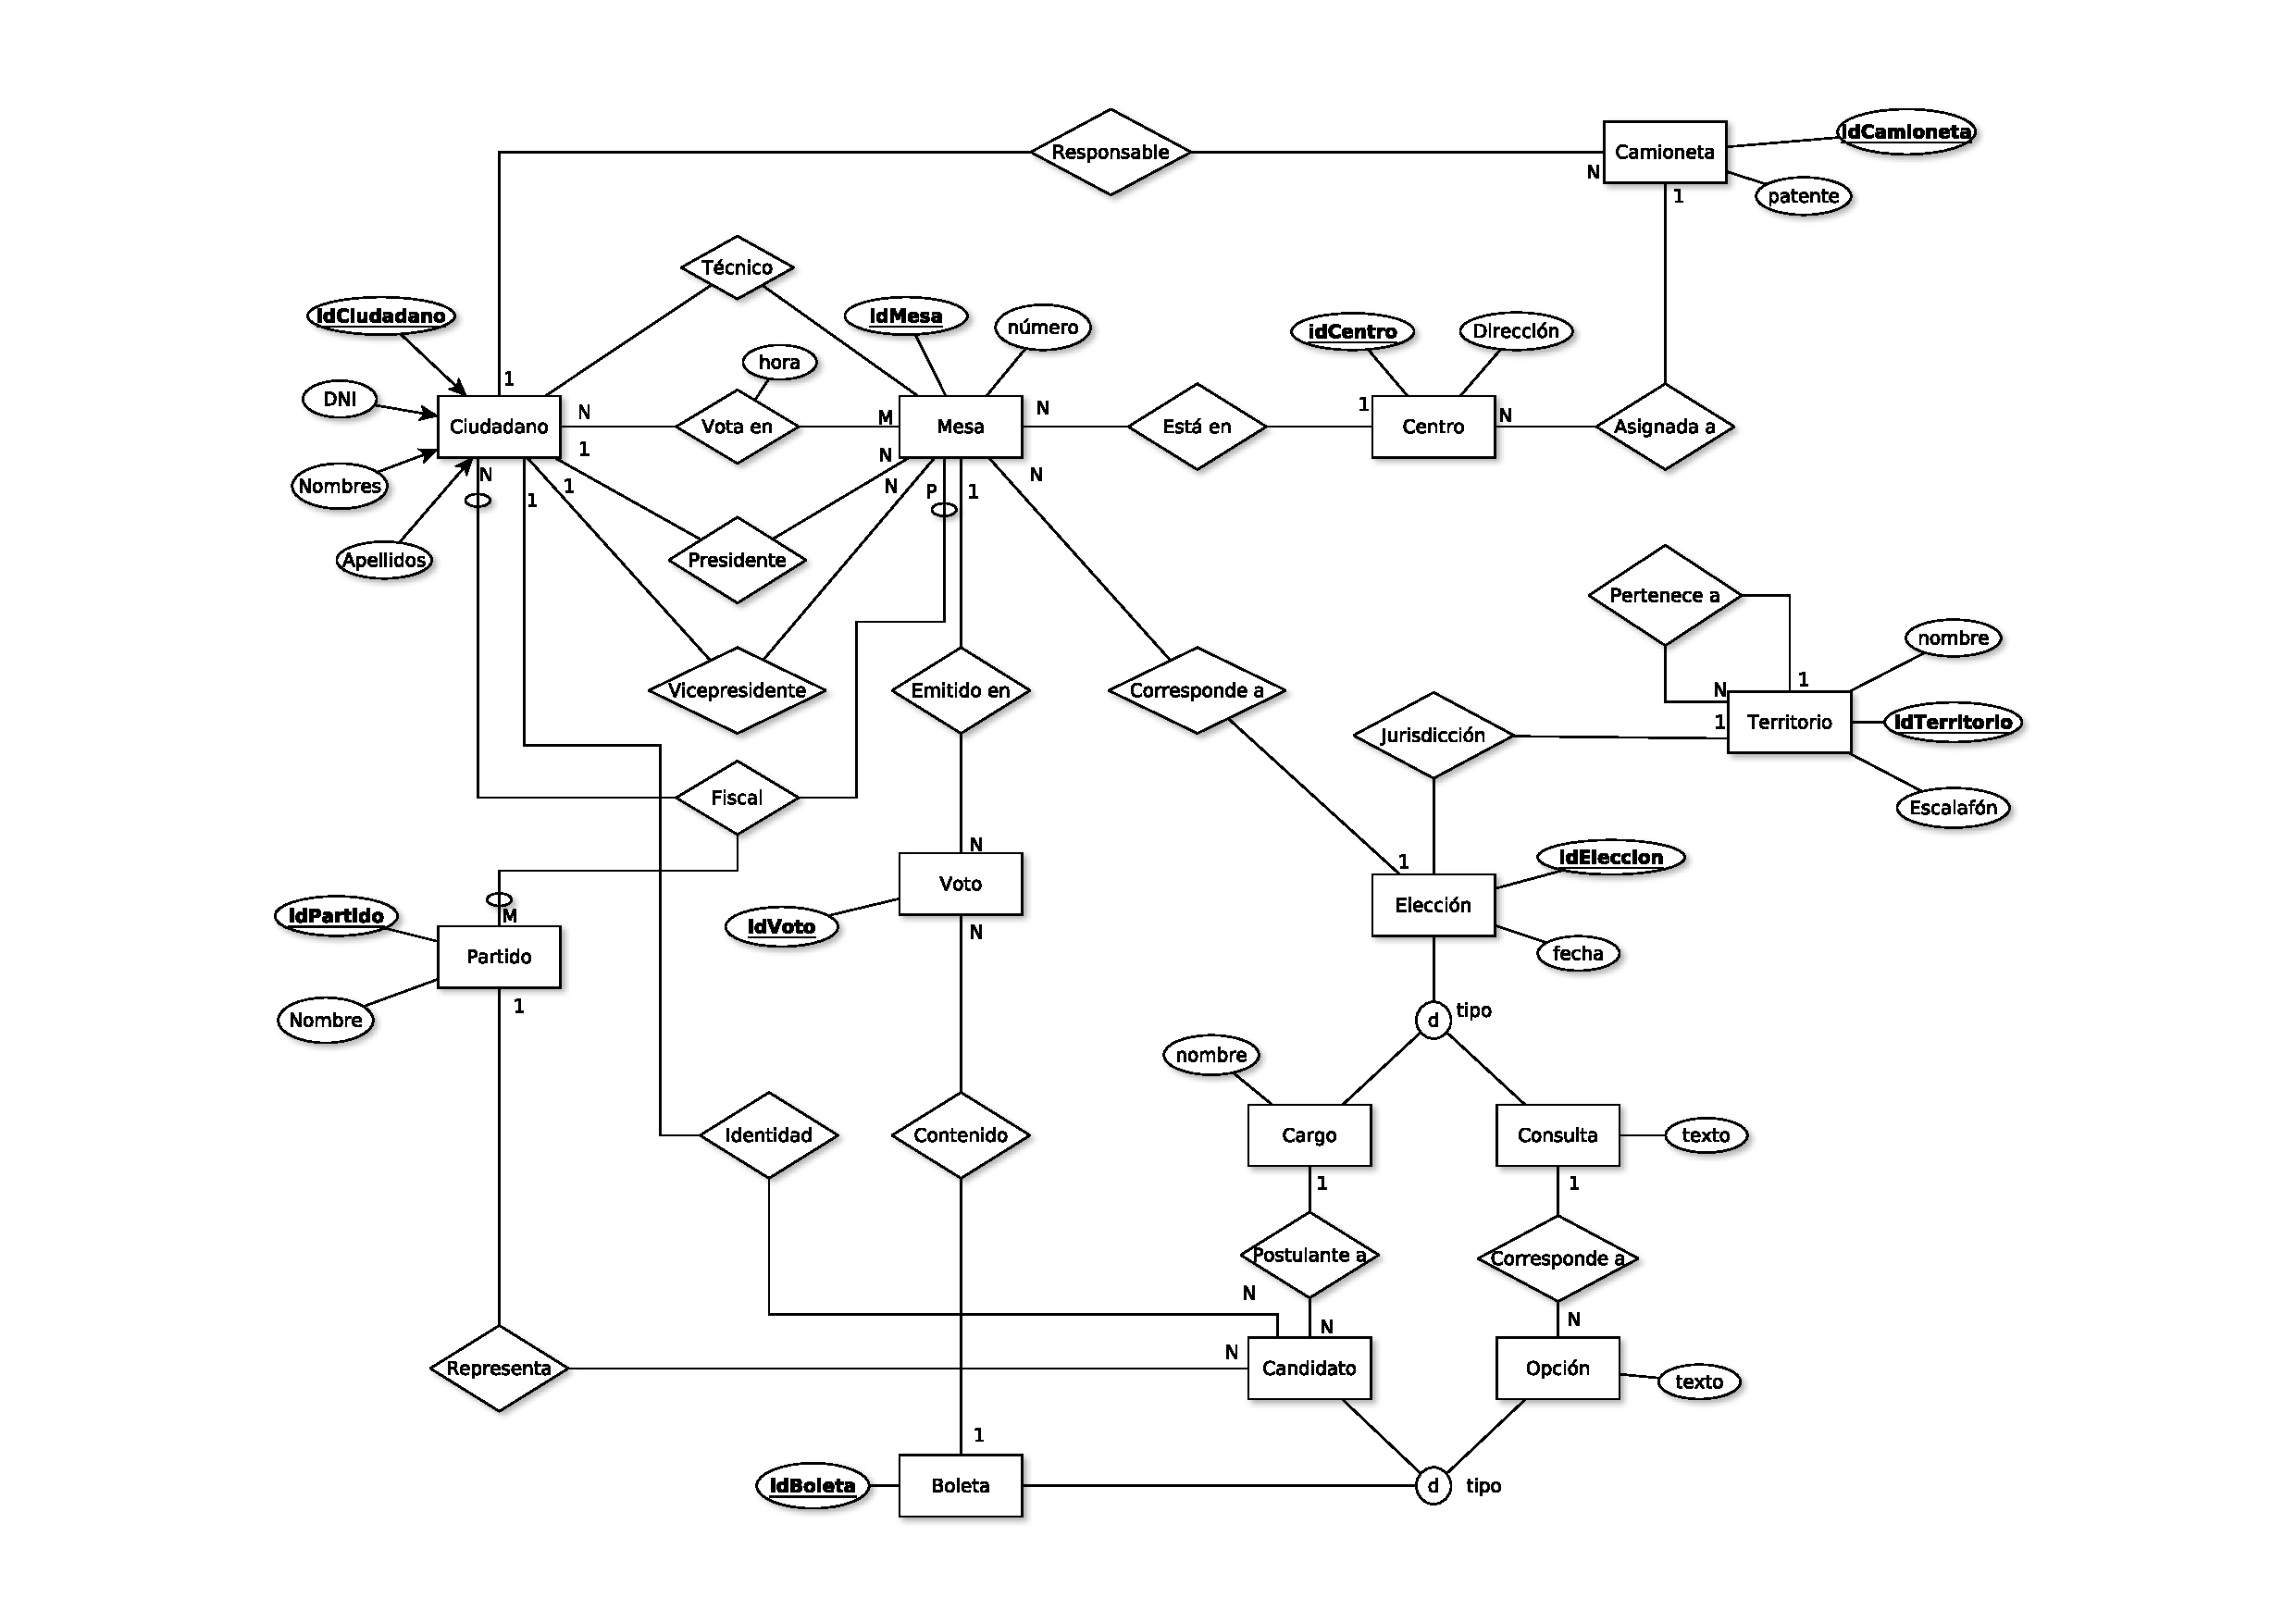
\includegraphics[scale=0.5]{DER.svg}
    %%\caption{Ejemplo sencillo}
\end{figure}

\subsection{Modelo Relacional}

\subsection{Restricciones adicionales}

\section{Implementacion}
\subsection{Stored Procedures}
% Acá irá el código lisa y llanamente

\section{Datos de testing}
\subsection{Scripts de carga de datos}



\end{document}
